%%%%%%%%%%%%%%%%%%%%%%%%%%%%%%%%%%%%%%%%%%%%%%%%%%
% This is the LaTeX file for the chapter:
% Blockchain Security
% for the manual:
% COMP716 - Highly Secure Systems
% Written by Jeff Nijsse
% September & October, 2018.
% Last updated Dec 10, 2018.
%%%%%%%%%%%%%%%%%%%%%%%%%%%%%%%%%%%%%%%%%%%%%%%%%%
%
\chapter{Blockchain \& Cryptocurrency}\label{Ch:BC}
The \defn{crypto} in cryptocurrency comes from cryptography; thus, a cryptocurrency is a currency that is cryptographically secured. In 2017 the term \defn{cryptocurrency} was added to the Oxford English Dictionary along with \defn{bitcoin} and \defn{blockchain}. This chapter will introduce the technology that enables bitcoin and some of the security implications of a blockchain based application. Blockchain and bitcoin have become synonymous but there are important differences. First we will look at the blockchain as a data structure.
%%%%%%%%%%%%%%%%%%%%%%%%%%%%%%%%%%%%%%%%%%%%%%%%%%%%%%%%%%%%%%%%%%%%%%%%%%%%%%%%%%%%%%%%%
%%%%% Blockchain Data Structure                                                     %%%%%
%%%%%%%%%%%%%%%%%%%%%%%%%%%%%%%%%%%%%%%%%%%%%%%%%%%%%%%%%%%%%%%%%%%%%%%%%%%%%%%%%%%%%%%%%
\section{Blockchain Data Structure}\label{Se:BCDataStructure}
A blockchain is a data structure whereby a single block of data contains a reference to a previous block. Usually this has occurred in the past, and so a chain of blocks can represent a chronological ordering of data. When a new block is created it must include a reference pointer to the previous block in the chain. This is done by including a hash of the previous block.
\begin{center}
\includegraphics[width=0.85\textwidth]{blockchain}
\end{center}
The blockchain must be created one block at a time and mass deletion or appending of new blocks is not possible to maintain the correct hash linking. If there are multiple new blocks to be added to the data structure, they must queue and be processed according to some predetermined rules. In this sense, a blockchain is considered to be immutable, and append-only. The first block, labelled ID:1 above, is often called the genesis block, and this is the only block that has been created by design at the inception of the program. All other blocks are added in sequence according to the protocol of the system.
 
Recall that a hash function takes a variable length input and produces a fixed length output with no discernible pattern. A good hash function is one-way which means that it is easy to calculate (verify) but difficult to reverse. Given a hash it should be computationally infeasible to both produce the data that created the hash, and to find a message that produces the same hash. This scenario is called a collision and for the blockchain to be secure it should be composed using a collision-resistant hash function.

If an adversary wishes to modify data in a block -- such as financial transaction data -- the resulting hash pointer will need to be updated. (Even a variation of a single bit yields a different hash.) So rather than having to store the entire data set for verification, we can store the hash pointers and easily see if they are correct. Our adversary that altered some data would have to change every subsequent hash pointer to the tip of the blockchain. Simply storing the most recent hash in a place that can't be modified is enough to verify the whole chain. This can be done by keeping multiple copies in different locations. 

\begin{center}
	\includegraphics[width=0.5\textwidth]{merkle}
\end{center}

The pages inside the books (data) can also be represented using hash pointers through a \defn{Merkle tree}, named after computer scientist and cryptographer Ralph Merkle. The leaves of the binary tree structure are the data and a hash pointer is created for every pair of leaves. When there are two pairs of leaves, the two hash pointers are combined and hashed into a third hash pointer. This continues until the root of the tree is a single hash representing all the data. The Merkle tree is secure in the same way as the blockchain -- if Eve tries to modify some data, then the root hash pointer will change. 

A blockchain data structure can be \defn{permissioned} and require some authentication to browse elements and append blocks, or \defn{permissionless} allowing anyone to view the data and perhaps add blocks depending on the rules of the protocol. There are applications for both styles of blockchain and, as many believe, currency works best as a public and transparent data structure.

%%%%%%%%%%%%%%%%%%%%%%%%%%%%%%%%%%%%%%%%%%%%%%%%%%%%%%%%%%%%%%%%%%%%%%%%%%%%%%%%%%%%%%%%%
%%%%% Cryptocurrencies                                                              %%%%%
%%%%%%%%%%%%%%%%%%%%%%%%%%%%%%%%%%%%%%%%%%%%%%%%%%%%%%%%%%%%%%%%%%%%%%%%%%%%%%%%%%%%%%%%%
\section{Cryptocurrencies}\label{Se:Cryptocurrencies}
Financial transaction data\footnote{Blockchains are sometimes called open ledgers in reference to an accounting ledger that tracks income and disbursements; similarly, distributed ledger technology refers to a blockchain combined with distributed computing architecture.} is an ideal use case for a blockchain data structure as it is generally chronological, and does not contain any cyclic elements (such as changing your name, which was appended to the database at birth). Hash pointers only work in a system like this because if a previous element changes, the subsequent hash pointers would need to be updated. Transactions themselves may be reversed, but from an  accounting perspective this is simply a debit back to the customer represented as a second transaction. Both transactions are stored and should be retrievable in the future.

A monetary system is an evolution of social trust. In small tribes or individual families, money is not necessary because the members trust each other to keep a tally\footnote{The term \emph{tally} comes from an old British system of keeping debts with notched wooden sticks called tallies.} of various debts and credits. In the case of a cryptocurrency, hash functions and public key cryptography allow a user to trust a stranger with their money. A monetary system can be constructed with a number of axioms.

Any monetary system must be:
	\begin{description}
	\item[Fungible] No single token is differentiable in value from another. Artwork exchange would be non-fungible because of the inherent personal differentiation of value.
	\item [Durable] The tokens must last at least long enough to be used in two transactions: one to receive them and one to spend them. This is solved easily with digital tokens.
	\item [Scarce] If everyone had easy access to it, it would not be valuable. This is a central problem with digital currency because copying digital entities results in a perfect duplicate indistinguishable from the original.
	\item [Divisible] Bartering with whole goods is difficult because value might not be aligned. This is a benefit of a digital system; coins can have a very high resolution, much greater than \$0.01.
	\end{description} 

A cryptographically secure financial transaction system should embody the following additional elements:
	\begin{description}	
	\item [Decentralization] Under control of the users; as opposed to the administrators. This helps ensure that value cannot be stolen, diluted, or written off by powerful actors in the system.
	\item [Uniqueness] Coins should only be allowed to be spent once. This is a key barrier to overcome when transacting in a digital medium.
	\item [Predictability of Supply] Creation and distribution of new tokens according to rules the users agree with. 
	\item [Distributed Network] The network should be invulnerable to attack or regulatory control from a single entity.
	\item [Security] Ownership of addresses (coins) and the ledger should be computationally secure and  hackers or bad actors should not be able to modify the historical record.
\end{description}

\subsection*{A Brief History: Before Bitcoin}
In 1983 David Chaum came up with a scheme for electronic cash involving distribution, tracking, and spending of coins that relied on a bank entity for clearing. Chaum's idea was to use what are called \defn{blind signatures} to keep the identity of the user hidden from the central clearing house, while still being able to trust that the hidden user had viable funds to spend. If the bank issues a new digital note to you and lets \textit{you} pick the serial number and then the bank signs it, there is now a new note in existence guaranteed by the bank but they don't know who they gave it to. If you tried to spend your new digital note twice the bank could step in and compare the transactions and call you out on the double-spend attempt.

Chaum started DigiCash in 1989 to allow users to conduct anonymous online transactions. DigiCash and others in the intervening years relied on banks for the issuance of new currency, and although had unique privacy features, banks largely did not need the new technology and did not adopt it. Much of the work since this time has involved trying to remove the bank from the equation to create a decentralized currency.  

Another issue to consider is the minting of the digital coins. A good solution requires a cost structure similar to the printing of modern notes where capital expenditure is large to acquire printing presses and develop the security features. This cost goes down over time as subsequent print runs cost less and less making it difficult for single users to print their own money. For digital minting, the computational power required to copy a digital serial number is negligent and so a more intensive process is required.

In 1997 original cypherpunk Adam Back came up with \defn{Hashcash}. Hashcash was developed to solve the problem of email spam. DDoS attacks on email servers can be mitigated by hashing a proof of computational effort and including it in the email header. Spammers and phishers must send thousands of emails to get a response and so a small delay in each mail sent can be very frustrating. The delay is negligible for the average user as their own processor could compute the proof-of-work during composing their message and not notice the cpu time required. The work that the cpu is doing is finding a solution to a hash puzzle. A variant of Hashcash is used in bitcoin and offers a solution to the coin minting problem. Section \ref{Se:POW} discusses proof-of-work.

%Hashcash is included in Linux distributions To invoke hashcash:
%\begin{code} terminal code to get some hashcash output
%\end{code}

%%%%%%%%%%%%%%%%%%%%%%%%%%%%%%%%%%%%%%%%%%%%%%%%%%%%%%%%%%%%%%%%%%%%%%%%%%%%%%%%%%%%%%%%%
%%%%% Bitcoin                                                                       %%%%%
%%%%%%%%%%%%%%%%%%%%%%%%%%%%%%%%%%%%%%%%%%%%%%%%%%%%%%%%%%%%%%%%%%%%%%%%%%%%%%%%%%%%%%%%%
\section{Bitcoin}\label{Se:bitcoin}
In 2008 a whitepaper emerged by Satoshi Nakamoto that combined many of the elements we have studied thus far and solved the double-spend problem in a distributed system. The new feature in bitcoin is called \defn{emergent consensus}\footnote{The term Nakamoto consensus is gaining popularity in the literature.} and allows a network of independent users and operators to monitor transactions against a global ledger. Every node independently verifies transactions and the network globally agrees on new blocks to be appended to the blockchain. This agreement of the blockchain state by its users is the last piece in the digital cash puzzle thereby eliminating the need for a trusted intermediary. Bitcoin tied together the following modules to create a distributed, cryptographically secure financial system:

\begin{description}
	\item [Decentralization] Bitcoin software is open-source so anyone can run the software and set up a node in the network. There has been considerable growth since 2009; estimates indicate there are around 10,000 full nodes online. Each node contains a copy of the blockchain and can independently validate transactions. This eliminates single-point-of-failure problems common in centralized systems.
	\item[Consensus] All participants must agree on the state of the ledger. It is this trust in the ledger that allows one party to interact with another that they did not previously know or trust personally. Sometimes this is referred to as \defn{trustless}.
	\item [Uniqueness] Every transaction has a hash pointer within a block. In this sense all the transactions are unique. Individual coins do not actually exist, rather hash pointers can indicate unspent transaction outputs that can show \begin{code}9.87654321 bitcoin\end{code}\footnote{A bitcoin is divisible into 8 decimal places; 0.000 000 01 is called a satoshi.}, for example. Whoever has the private key to these unspent outputs is considered the owner.
	\item [Supply Stability] Every block that is added to the chain results in the minting of new bitcoins. This amount is halved about every four years so the total supply is a decreasing geometric series. The maximum number of bitcoins that will be minted is just under 21 million.
	\item [Security] Bitcoin uses the NIST specification \begin{code}secp256k1\end{code} elliptic curve digital signature algorithm. This keeps users private keys secure and authenticates transactions in the network.
 
\end{description}
How do you keep the state of the whole blockchain safe from sticky fingers? What if one party decides to spend their coins to buy some gold, and then after receiving the gold, they spend their coins \textit{again}, this time sending them to another address they control. We need a way to distinguish between the two transactions without mediation. The next section will discuss this issue: how can everyone agree on what transaction is valid?

%%%%%%%%%%%%%%%%%%%%%%%%%%%%%%%%%%%%%%%%%%%%%%%%%%%%%%%%%%%%%%%%%%%%%%%%%%%%%%%%%%%%%%%%%
%%%%% Blockchain Consensus                                                          %%%%%
%%%%%%%%%%%%%%%%%%%%%%%%%%%%%%%%%%%%%%%%%%%%%%%%%%%%%%%%%%%%%%%%%%%%%%%%%%%%%%%%%%%%%%%%%
\section{Consensus}\label{Se:Consensus}
Solving the situation described above, known as the \defn{double spend problem}, is the final piece of the puzzle that was put in place for trustless decentralized digital cash to succeed. First we will describe the \defn{Byzantine Generals Problem}, a famous computer science communication problem. 

Imagine three generals of the same army, all wanting to attack an enemy fortress at dawn the next morning. Each general knows their individual divisions cannot win the enemy fortress. Each general also knows that with the help of the other's forces they can win the position. So General \textit{Alpha} sends a messenger to General \textit{Beta} with the message ``We attack at dawn.'' This is where the problems start. There are many scenarios that could play out. The messenger could be captured by the enemy; the messenger could be a double-agent; the messenger could get lost and not deliver the message; General Beta could double-cross Alpha, etc. To win the battle, the three generals must come to consensus and agree to attack at dawn. Practically speaking, each general must receive confirmation from each of the other generals that they received the message \emph{and} are in agreement. This scenario maps nicely onto cryptography and message passing.
%distributed consensus state diagram 
\begin{center}
	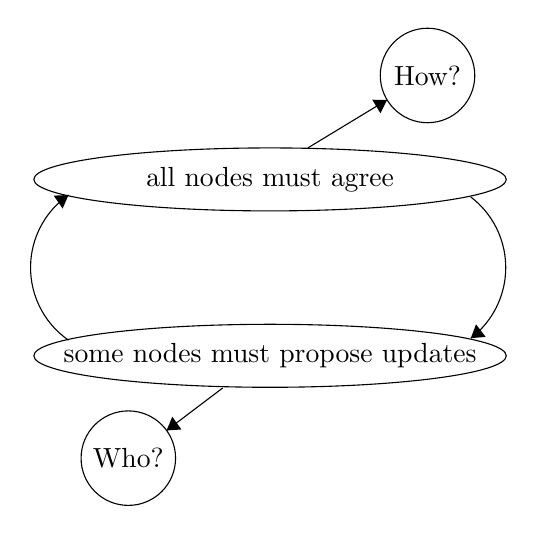
\begin{tikzpicture}[scale=0.2]
	\tikzstyle{every node}+=[inner sep=0pt]
	\draw [black] (35,-20.2) ellipse (15 and 2);
	\draw (35,-20.2) node {all nodes must agree};
	\draw [black] (35,-31.4) ellipse (15 and 2);
	\draw (35,-31.4) node {some nodes must propose updates};
	\draw [black] (45,-13.6) circle (3);
	\draw (45,-13.6) node {How?};
	\draw [black] (26,-37.9) circle (3);
	\draw (26,-37.9) node {Who?};
	\draw [black] (22.205,-30.413) arc (-124.75549:-235.24451:5.615);
	\fill [black] (22.2,-21.19) -- (21.26,-21.23) -- (21.83,-22.05);
	\draw [black] (47.747,-21.315) arc (52.66893:-52.66893:5.64);
	\fill [black] (47.75,-30.28) -- (48.69,-30.2) -- (48.08,-29.4);
	\draw [black] (37.4,-18.2) -- (42.43,-15.15);
	\fill [black] (42.43,-15.15) -- (41.49,-15.14) -- (42.01,-16);
	\draw [black] (32,-33.44) -- (28.43,-36.14);
	\fill [black] (28.43,-36.14) -- (29.37,-36.08) -- (28.79,-35.27);
	\end{tikzpicture}
\end{center}
A decentralized blockchain application has many nodes in the network and each of them has a copy of the blockchain. If Bob wants to send Alice his tokens, the nodes in the network must first agree that Bob has available tokens to spend, and then update the state before Bob can double-spend his tokens. The network needs to be in a state of \defn{consensus} for people to trust it. Consensus in the Byzantine Generals problem has been proven to be impossible if more than a third of the nodes are malicious.\footnote{The term Byzantine in computer science indicates an unpredictable actor--this includes malicious activity.}

Bitcoin does not exactly mirror the model of the Byzantine Generals and so is not impossible to reach consensus. In other words, bitcoin does achieve consensus despite Byzantine behaviour. More practically, bitcoin achieves a state of \textit{emergent} consensus. This means that over time as blocks get added to the chain, a general state emerges that everyone agrees on. So how does this occur without clear rules? A closer look at the double-spend attack will illustrate how nodes come to agreement.

\subsubsection*{The Double-Spend Attack}
A dodgy actor, Eve, could manipulate the blockchain by sending some coins to Jeff and receiving a good or service. Then she could send those same coins to Bob's address whom she also controls. If the transaction involving Bob's address is validated on the blockchain, then Eve would have successfully double-spent the same coins. She now has the coins in Bob's address and the goods from the transaction with Jeff.\\
\begin{center}
\includegraphics[width=0.8\textwidth]{doubleSpendSuccess}
\end{center}
How can Jeff avoid this scenario, especially when he does not know the other party he is transacting with? The solution is to wait. Over time as more blocks are added, say every ten minutes, the older blocks are more likely to be valid.\footnote{Standard confirmation time for bitcoin is six blocks, or one hour. The number of blocks to wait until considering a transaction to be confirmed is a personal preference.} Stated another way, as more blocks are added to the chain there is an exponential decrease in the probability of a block being rejected by other nodes. This is the method that secures the blockchain against malicious nodes attempting to double spend. 

\begin{center}
	\includegraphics[width=0.8\textwidth]{doubleSpendSolution}
\end{center}

And what about Eve changing history? She would have to alter the block where the transaction is stored, as well as any subsequent blocks. The older the block is, the more computational effort is required because the hash pointers are linked. Consider that Eve is also competing against other nodes in the network that are honest. (We will return to the case of dishonest nodes when discussing a 51\% attack.) The next question is how to keep nodes honest, especially when dealing through the medium of currency? 

\subsection*{Proof-of-Work}\label{Se:POW}
Here is an important distinction where bitcoin varies from other methods of reaching consensus. There are incentives for nodes to act honestly that are built into the protocol. The first is called the \defn{coinbase} transaction and awards freshly minted bitcoins to whoever added the block to the chain. This is how new bitcoins come into circulation. The second is from transactions fees. By listening to the network, validating transactions, and including them in a block, whoever is operating the node can choose to include transactions that also offer an extra fee. Because bitcoin itself is designed to be digital money, this makes perfect sense and is why cryptocurrency is considered the killer app for blockchain. 

Referring back to the state diagram, who gets to propose these blocks and earn the block reward? How do we ensure the distribution is random? How are Sybil attacks prevented? Mining is the answer and provides the incentive structure to maintain this delicate balance.

\subsubsection*{Mining}
A miner is a network participant that contributes their computing power in a demonstrable way. A fair way to allocate the incentives would be by some resource that can not be gamed or monopolized. One such way is by computing power, and is called \defn{proof-of-work}. Another method is by value held in reserve and is called proof-of-stake. Proofing methods is a very active research topic as it has many game theoretic variables.\footnote{Other methods include DPoS: delegated proof-of-stake, PoET: proof of elapsed time, and PoA: proof of authority.} Bitcoin miners participate by using their computing power to validate transactions and suggest new blocks. For this effort they receive rewards in proportion of their contribution to the network as a whole. Bitcoin uses a \begin{code}SHA256\end{code} hashing algorithm as the hash puzzle that miners have to find a solution for.
\begin{center}
\begin{code}
	Block = Hash(nonce||previousHash||data||data||...||data) < target
\end{code}
\end{center}

 Hash function output has a random distribution and so to find a block, your hash must be below a certain target level. The target level will be the hash size with a certain number of leading zero bits, for example:\begin{center}\begin{code}
	000000000000000000117c467ab5336077cb04f7f70ea6ebcd68e0b3ef6cf909
\end{code}\end{center} 
was the successful hash of block \begin{code}529283\end{code}. The only way to find a hash with a smaller value than the target is to change a nonce value and re-hash the bundle of transactions over and over. When a target is hit, the block is broadcast to the network as a proof of computational work done in solving the hash puzzle. 
The bits here should be randomly distributed, like a lottery, to prevent gaming the system and earning more rewards than your proportion\footnote{As the bitcoin network has matured, dedicated hardware called ASICs (application specific integrated circuits) to solve the \begin{code}SHA256\end{code} algorithm have dominated. It is no longer feasible for a single participant to mine bitcoin without dedicated hardware.}. Computing cycles in the bitcoin network is called \defn{hashpower} in reference to \begin{code}SHA256\end{code}. As more miners come online, the total hashpower increases leading to greater overall probability of successfully hashing a value below the target. To keep the temporal distribution of blocks even, this target difficulty automatically adjusts according to the protocol every 2016 blocks, or approximately two weeks.

Below is a log plot of the mining difficulty from 2009-2018 showing that the difficulty has increased exponentially. The slope roughly correlates to the growth of the network.\footnote{Source: \url{https://www.blockchain.com/charts/difficulty}}

\begin{center}\vspace{0.3cm}
	\includegraphics[width=1.0\textwidth]{difficulty}
	% source https://www.blockchain.com/charts/difficulty
\end{center}

\subsubsection*{Block Time}
The difficulty adjustment aims to keep the time between blocks (successful hashes) at around ten minutes. In the early days Satoshi and a few others could use their PC processors to find blocks every ten minutes. The hashpower has steadily increased and so has the difficulty target to keep the block time constant. Finding a hash of a block that is below the target size is a discrete event; it is either below or it is not. As with a lottery, it is only a matter of time before a hash is found, and the previous hash is independent of the current attempt. Statistically, this is a \defn{Poisson} distribution. %The probability of a block being found is $P(N)=1-e^{-1}$

\begin{center}
	\includegraphics[width=0.85\textwidth]{blockTimePoisson}
	% source https://en.bitcoin.it/wiki/Confirmation
\end{center}

From the graph\footnote{Source: \url{https://en.bitcoin.it/wiki/Confirmation}} you can see its possible to find a block immediately after the last one, but unlikely. Similarly, its possible that no block could be found for an hour or two, but unlikely. In practice, the average block time is just under ten minutes because as more miners join the network it is easier overall to find blocks, until the difficultly is reset. 

\subsubsection*{Consensus Summary}
In summary, consensus of nodes in the network emerges from an implicit agreement on the longest chain of blocks. The nodes are all agreeing that this blockchain represents the most proof of computational work. Miners will abandon shorter chains to compete to build on the longer one to win the block reward. The transactions in this chain will have an increasing probability of being accepted over time as new blocks are mined. 

%%%%%%%%%%%%%%%%%%%%%%%%%%%%%%%%%%%%%%%%%%%%%%%%%%%%%%%%%%%%%%%%%%%%%%%%%%%%%%%%%%%%%%%%%
%%%%% Blockchain Security Considerations                                            %%%%%
%%%%%%%%%%%%%%%%%%%%%%%%%%%%%%%%%%%%%%%%%%%%%%%%%%%%%%%%%%%%%%%%%%%%%%%%%%%%%%%%%%%%%%%%%
\section{Security}\label{Se:BCSecurity}
The first security consideration was the double-spend attack as discussed above. The next weakness comes at the network level. To this point we have said that most nodes in the network will act honestly and the mining block reward incentivises this behaviour. If a collective forms with a considerable portion of nodes this could lead to a 51\% attack.

\subsubsection*{51\% Attack}\label{Se:51}
Should a single entity gain control of more than half of the hashpower in the network, this could lead to a 51\% attack. The attacker can't steal coins directly as this involves subverting elliptic curve cryptography. The attacker can however user their majority status in some interesting ways. At $>50\%$ you have the ability to find more blocks and direct consensus of the blockchain. The attacker can censor transactions by refusing to add blocks containing someone's address. This would be akin to blacklisting certain addresses, but does not completely exclude these from being included by honest nodes (the 49\%). Next, you may say okay, lets just increase the block reward and award myself 1 million coins for the next block found. This will be rejected by the network because the block reward is hard-coded and so the malicious ``plus-one-million'' transaction can never be spent. 

An adversary doesn't necessarily need 51\% of the hashpower, but with a large number of nodes in the network they could facilitate a double spend attack by the following steps.
\begin{enumerate}
	\item Broadcast a transaction they intend to double spend that the receiver believes is legitimate.
	\item Mine a different branch of the blockchain that doesn't include their transaction from (1), but does include a transaction to themselves.
	\item Continue mining the forked branch until the illegitimate transaction is accepted by the receiver and then broadcast their alternate blockchain.
	\item As consensus relies on the longest chain representing the most proof of work, this new (and falsified) chain will now be considered valid.
\end{enumerate}

The main practical threat to a single entity controlling the majority of the hashpower is that it will lead to centralization and cause users to abandon the system altogether. Once hashpower gets close to this threshold it is also possible that developers will step in and update the software to limit this behaviour. It is unknown how this will play out in the future. Thus far the bitcoin network has been relatively decentralized, but a few mega mining companies have emerged. There have been some cases of 51\% attacks on alternative cryptocurrencies such as Verge, Horizen, and Vertcoin. Smaller cryptocurrencies are more vulnerable to a large mining pool shifting their resources for this purpose.

\subsubsection*{Cryptography}\label{Se:bitcoinCryptography}
Contrary to popular belief there is no standardized encryption in the bitcoin protocol. As a decentralized system of exchange, there is no need for encryption. All the transactions are stored in the blockchain and accessible to everyone. Access to the private keys controlling addresses is maintained solely through personal security of the user. 

So can someone steal my coins? Not by hacking. Elliptical curve cryptography keeps keys safe from cryptanalysis via the difficulty in solving the discrete logarithm problem. The standard curve \begin{code}secp256k1\end{code} was chosen by the designer of the bitcoin protocol. This is a choice unique to bitcoin, as the more common \begin{code}secp256r1\end{code} is used in Transport Layer Security (TLS) for web browsing, email, etc., and discussed in Section 2.4. ECC was chosen because it provides the same level of relative security with smaller keys compared to RSA.

It is imperative that users keep their private keys secret as in any other cryptosystem. There are some added enhancements for encrypting passwords and wallets but these are third party additions and not built in to the protocol.

\subsubsection*{Key Storage}
Storage of cryptocurrency is similar to storage of your online banking details. There are no actual bitcoins to keep safe; there is no \begin{code}<bitcoin object>\end{code} to keep password protected. Remember the blockchain is an open ledger of every transaction in the network. Just like your online banking system keeps track of all account balances and doesn't actually store any fiat\footnote{Fiat is government issued money. New Zealand dollars and Japanese yen are both considered fiat currency.}. Bitcoin is cryptographically secured, and if you have the private keys to an address, then you control the funds that address references in the blockchain. 

A bitcoin address is the public key of a public-private key pair generated by a 256 bit elliptic curve function. The public key is encoded in base-58 to reduce errors in transcription by removing similar characters: \begin{code}0O1l\end{code}.
\begin{center}
	\includegraphics[width=0.65\textwidth]{keysQR}\end{center}
% source bitcoin presentation
Cryptocurrencies are more risky than traditional online banking because if you lose your private keys they are not recoverable. There is no password reset, or government issue ID verification to recover your account. 

There are a number of way to store your keys:
\begin{description}
	\item[Hot Wallet] This is the most common. A software application that stores your private keys so you can sign transactions, keeps track of your tokens, and maybe offers some additional functionality like multiple addresses, or multiple token support. The risk here is that if you lose your device, your private keys are gone with it. Day-to-day transactions using a smartphone would be done through a hot wallet.
	\item[Cold Storage] For larger amounts, savings, investments, and custodial services, a cold wallet is recommended. This is a device that is not powered and has no connectivity and stores your private keys internally. When tokens are required, it can be plugged into a USB and connected to the network. 
	\item[Paper Wallet] Once a key pair has been generated and used to receive tokens, that private key will always have ownership of the tokens. The private key can be printed out or written down, sometimes as a QR code for easy scanning. After the memory has been cleared there is no more digital record of the private keys.
	\item[Brain Wallet] The most hard-core of storage systems is to remember your private keys and destroy all physical and digital evidence of them. Certain memory mnemonics can help with this. 
\end{description}	
Note that for all these methods including memorization, its possible to \textit{send} tokens to your address without connecting the keys to the network. This transaction will be recorded by all the nodes running the blockchain and propagated accordingly. Private keys are only required to sign transactions (spend tokens). All of these methods are vulnerable to crisis such as fire or theft, and represent a single point of failure. Backing up your keys can solve the crisis issues, but someone could still steal the backup. 

\subsubsection*{Secret Sharing}
Lets assume that eventually someone \textit{will} steal our private keys. In this scenario they need the entire key, in the correct order to use it. So why not split the key in two or several parts? This is known as \defn{secret sharing} and works like this: split the key into $N$ shares such that any $K$ of those shares can reconstruct the key, but with $<K$ shares nothing can be learned. Lets split the secret $S$  into 2 shares so that $N=2$ and $K=2$. If $S$ is a 128 bit number, a random 128 bit number $R$ is generated and the 2 shares can be $R$ and $S\oplus R$ (bitwise XOR). Either share alone does not help because $R$ is random, and $S\oplus R$ depends on knowing $R$. In essence the secret has been encrypted with a one-time pad cipher where $R$ is the key. This works for $N=K$. What about for $N>K$?

Say you split the secret in to four shares, give one to each of your trustworthy relatives, and at any time two of them are required to reconstruct the secret. This can be accomplished with some linear algebra. Any two points can construct a line, but given a third random point it is unlikely to be collinear with the first two. To generate $N$ shares, prepare a line with $N$ points. Now any two of these points can reconstruct the line, and determine the $x-$intercept ($S$), but any single point is useless because the slope is unknown. 

\begin{center}
	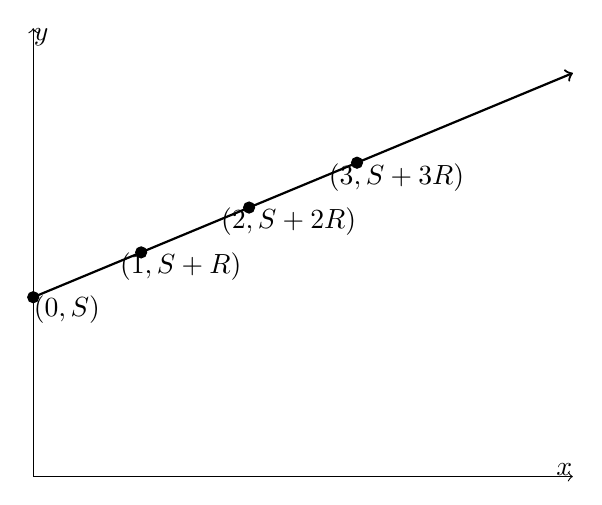
\begin{tikzpicture}
	\pgfplotsset{ticks=none}
	\begin{axis}
	[grid=none,
	scale=1,
	xmin=0, xmax=5,
	ymin=0, ymax=2.5,
	axis lines=middle,
	axis line style={->},
	xlabel=$x$,
	ylabel=$y$,
	]
	\addplot[->,domain=0:5,samples=50,smooth,thick,black] {0.25*x+1};
	\addplot[mark=*, nodes near coords={$(0,S)$},every node near coord/.style={anchor=160}] coordinates {(0,1)};
	\addplot[mark=*, nodes near coords={$(1,S+R)$},every node near coord/.style={anchor=160}] coordinates {(1,1.25)};
	\addplot[mark=*, nodes near coords={$(2,S+2R)$},every node near coord/.style={anchor=160}] coordinates {(2,1.5)};
	\addplot[mark=*, nodes near coords={$(3,S+3R)$},every node near coord/.style={anchor=160}] coordinates {(3,1.75)};
	\end{axis}
	\end{tikzpicture}
\end{center}

The point $(0,S)$ represents the secret, a large random number less than a large prime, $P$. The shares are linear combinations modulo $P$, up to $N$, where any 2 of them will recover the secret.
\begin{align*}
x=0,\quad y&=S\\
x=1,\quad y&=(S+R)\mod P\\
x=2,\quad y&=(S+2R)\mod P\\
x=3,\quad y&=(S+3R)\mod P\\
\vdots\\
x=N,\quad y&=(S+NR)\mod P\\
\end{align*}
What if you require more than 2 shares necessary to reconstruct the key? If we increase the degree of our share-reconstruction function from linear to parabolic, then we have $K=3$ is necessary to find $S$ because 3 points can uniquely define a parabola. This can be continued up to $K=N-1$ shares.



%%%%%%%%%%%%%%%%%%%%%%%%%%%%%%%%%%%%%%%%%%%%%%%%%%%%%%%%%%%%%%%%%%%%%%%%%%%%%%%%%%%%%%%%%
%%%%% Privacy                                                                       %%%%%
%%%%%%%%%%%%%%%%%%%%%%%%%%%%%%%%%%%%%%%%%%%%%%%%%%%%%%%%%%%%%%%%%%%%%%%%%%%%%%%%%%%%%%%%%
\section{Privacy}\label{Se:Privacy}
Identity in a decentralized system is based on private keys. Whoever has access to a private key can operate within the network and this activity is directly linked to the key. Just like how digital signatures provide non-repudiation, the activity of an address within an open ledger can be thought of as someone's identity. Keeping with this idea of keys as identities, multiple keys could be multiple identities. You could generate a new identity with a new random key pair and never use the old identity again. 

There is a problem here if you want to remain anonymous. Anonymity means that you can still participate in the network but it is difficult or impossible to link your activity with your real identity. Even if one user has multiple addresses, the activities of those addresses is stored in the open -- every node in the network has a copy. For this reason, bitcoin is considered to be \defn{pseudonymous}. The activity of one address can be tracked, and this can be mapped to behaviour, possibly providing compelling evidence to link the two. Privacy in cryptocurrencies is a contentious issue and often cited as a founding principle. It goes right back to the core tenet of cryptography -- communicating in secret. For a user of cryptocurrency this may be as innocent as purchasing a VPN to use the internet where content and websites may be censored, or for much more nefarious purposes.\footnote{For many years bitcoin was synonymous with the \defn{Silk Road}, an online marketplace that remained out of reach of authorities and sold illegal goods. The possibility to purchase illegal material is still a main point of debate against cryptocurrencies. Many people have studied anonymity in markets and cash is still the best way to transact without revealing your identity.}

Coin mixing or laundry services aggregate transactions together and wash by sending a large transaction to one or many addresses controlled by the service. Funds are then returned less a service fee. This will help to obfuscate origin and destination of funds from forensic analysis but requires a large amount of trust in the mixing service. This is a weak and impractical solution to transaction anonymity. 

\subsubsection*{Zero-Knowledge Proofs}
Privacy can be built in cryptographically at the protocol level using a technique called \defn{zero knowledge}. In cryptography, zero-knowledge proofs are a way to mathematically prove that you know a result without having to reveal the details of how you found it. An example comes from mining. You can prove to someone that you have the hash of a block by revealing the nonce and therefore give away the formula for how you found the hash. A zero-knowledge proof lets you do this without revealing the nonce. The details are non-trivial and out of the scope of the present course. Refer to Foundations of Cryptography by Oded Goldreich, 2001, for an overview.

Several alternative cryptocurrencies have implemented zero-knowledge proofs such as Z-Cash, Horizen, and Ethereum's Byzantium upgrade. These are not compatible with bitcoin as a different set of cryptographic principles had to be coded from the beginning. In Z-Cash, which was derived from zerocoin, the user has the option to transact privately by invoking zero knowledge verification. This takes extra computational resources and reduces efficiency representing a trade-off between privacy and speed.


%%%%%%%%%%%%%%%%%%%%%%%%%%%%%%%%%%%%%%%%%%%%%%%%%%%%%%%%%%%%%%%%%%%%%%%%%%%%%%%%%%%%%%%%%
%%%%% Code-Breaking                                                                 %%%%%
%%%%%%%%%%%%%%%%%%%%%%%%%%%%%%%%%%%%%%%%%%%%%%%%%%%%%%%%%%%%%%%%%%%%%%%%%%%%%%%%%%%%%%%%%
\section*{Code-Breaking}\label{Se:code-breaking}
In October, 2018, an image was posted online claiming to contain clues to unlock a wallet holding 310 bitcoin (at the time of writing worth \$2.9 million NZD). Just days later the coins were moved from the wallet indicating the private keys had been found in the image. The image below contains a total of four keys, and one with 0.31 bitcoin is still unclaimed. A high resolution image can be downloaded at \url{https://bitcoinchallenge.codes/}.
\begin{center}
	\includegraphics[width=1.0\textwidth]{BTCchallenge}
	% source https://bitcoinchallenge.codes/
\end{center}
%
%
%
%
% \\END Blockchain
